\section{Problem representation}
Before a solution for the problem formulation can be designed, the problem domain must be more precisely defined, so it is clear what the system needs to know about, and consequently a model for representing the problem can be proposed. This section describes the problem domain and a fitting model of the problem domain.

\subsection*{Domain}
\figref{fig:problem-domain} illustrates the problem domain. 
\begin{figure}[h!]
  \centering
    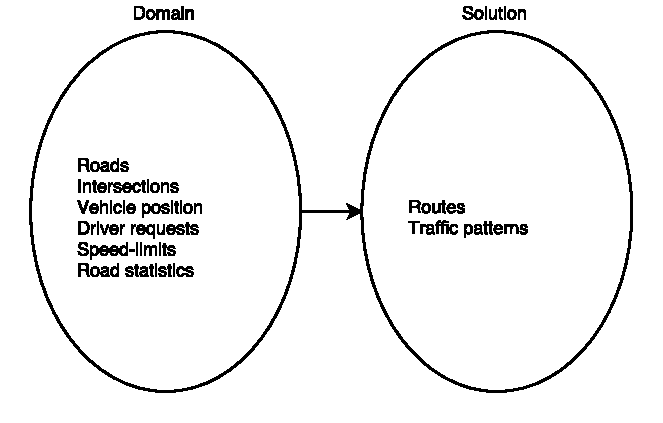
\includegraphics[width=0.8\textwidth]{figures/pd.pdf}
    \caption{Problem domain}
    \label{fig:problem-domain}
\end{figure}
\todo{Discuss and review this figure}
The problem domain consists of roads, intersections and vehicle positions a road network as well as the requirements of drivers of vehicles. The roads also include properties of said roads, such as the traffic, speed-limits and other relevant statistics about the road network. Most of these properties can be inferred from the traffic history of a given e.g. the usual speed of vehicles on that road.\todo{review the wording of the section}

\subsection*{Model}
To represent the problem domain we model the problem as a weighted, directed graph. \\
Let G be a weighted directed graph $G(N,E)$ where $E$ is the set of edges corresponding to roads between intersections and $N$ is the set of nodes corresponding to intersections of roads. Each edge $e_i \in E$ is a tuple $(n_o, n_t)$ where $n_o, n_t \in N$ and represents the direction of an edge from the origin node, $n_o$ to the target node $n_t$. Each edge also has an associated cost, $c(e_i)$ where  $c: E \rightarrow \mathbb R_+$ is the cost function. The cost of each edge describes the preference of taking the particular road corresponding to the edge. 

We want to design an algorithm for the cost function, that dynamically change the cost for each edge, as the flow of traffic in the road network changes, such that better routes dynamically can be determined based on the current traffic situation.\todo{discuss describing the cost function here versus other place}

\subsection*{Constraints(?)}
Here we define the constraints on the model from the problemformulation.